% (find-LATEX "2020-2-C2-edovs.tex")
% (defun c () (interactive) (find-LATEXsh "lualatex -record 2020-2-C2-edovs.tex" :end))
% (defun C () (interactive) (find-LATEXsh "lualatex 2020-2-C2-edovs.tex" "Success!!!"))
% (defun D () (interactive) (find-pdf-page      "~/LATEX/2020-2-C2-edovs.pdf"))
% (defun d () (interactive) (find-pdftools-page "~/LATEX/2020-2-C2-edovs.pdf"))
% (defun e () (interactive) (find-LATEX "2020-2-C2-edovs.tex"))
% (defun o () (interactive) (find-LATEX "2020-2-C2-edovs.tex"))
% (defun u () (interactive) (find-latex-upload-links "2020-2-C2-edovs"))
% (defun v () (interactive) (find-2a '(e) '(d)))
% (defun d0 () (interactive) (find-ebuffer "2020-2-C2-edovs.pdf"))
% (defun cv () (interactive) (C) (ee-kill-this-buffer) (v) (g))
%          (code-eec-LATEX "2020-2-C2-edovs")
% (find-pdf-page   "~/LATEX/2020-2-C2-edovs.pdf")
% (find-sh0 "cp -v  ~/LATEX/2020-2-C2-edovs.pdf /tmp/")
% (find-sh0 "cp -v  ~/LATEX/2020-2-C2-edovs.pdf /tmp/pen/")
%     (find-xournalpp "/tmp/2020-2-C2-edovs.pdf")
%   file:///home/edrx/LATEX/2020-2-C2-edovs.pdf
%               file:///tmp/2020-2-C2-edovs.pdf
%           file:///tmp/pen/2020-2-C2-edovs.pdf
% http://angg.twu.net/LATEX/2020-2-C2-edovs.pdf
% (find-LATEX "2019.mk")
% (find-CN-aula-links "2020-2-C2-edovs" "2" "c2m202edovs" "c2evs")

% «.videos»			(to "videos")
% «.video-1»			(to "video-1")
% «.video-2»			(to "video-2")
% «.defs»			(to "defs")
% «.title»			(to "title")
% «.introducao»			(to "introducao")
% «.campos-dirs»		(to "campos-dirs")
% «.exercicio-1»		(to "exercicio-1")
% «.exercicio-2»		(to "exercicio-2")
% «.como-testar-sols»		(to "como-testar-sols")
% «.como-testar-uma-sol»	(to "como-testar-uma-sol")
% «.exercicio-3»		(to "exercicio-3")
% «.exercicio-4»		(to "exercicio-4")
% «.exercicio-5»		(to "exercicio-5")
%
% «.djvuize»			(to "djvuize")

% «videos»  (to ".videos")
% (c2m202edovsa  "videos")

% «video-1»  (to ".video-1")
% (c2m202edovsa   "video-1")
% (find-ssr-links     "c2m202edovs" "2020-2-C2-edovs" "bNfZUomf1xg")
% (code-eevvideo      "c2m202edovs" "2020-2-C2-edovs" "bNfZUomf1xg")
% (code-eevlinksvideo "c2m202edovs" "2020-2-C2-edovs" "bNfZUomf1xg")
% (find-c2m202edovsvideo "0:00")
% (find-c2m202edovsvideo "5:54" "a gente vai interpretar esse f'(x)")
% (find-c2m202edovsvideo "6:30" "desenhando os coefs angs só desses 10 pontos daqui")
% (find-c2m202edovsvideo "7:37" "Exercício 1")
% (find-c2m202edovsvideo "8:10" "figuras do Thomas")
% (find-c2m202edovsvideo "9:10" "ele faz vários desenhos")
% (find-c2m202edovsvideo "9:30" "aqui vocês vão fazer 7 desenhos diferentes")
% (find-c2m202edovsvideo "10:50" "quais dessas curvas parecem ser soluções")

% «video-2»  (to ".video-2")
% (c2m202edovsa   "video-2")
% (find-ssr-links     "c2m202edovs2" "2020-2-C2-edovs-2" "Ejr2wvpBiTE")
% (code-eevvideo      "c2m202edovs2" "2020-2-C2-edovs-2" "Ejr2wvpBiTE")
% (code-eevlinksvideo "c2m202edovs2" "2020-2-C2-edovs-2" "Ejr2wvpBiTE")
% (find-c2m202edovs2video "0:00")
% (find-c2m202edovs2video "0:50" "como se a gente ainda não soubesse o caso geral")
% (find-c2m202edovs2video "8:25" "eu vou traduzir dy/dx=-x/y pra")
% (find-c2m202edovs2video "8:44" "a gente quer uma solução que obedeça")
% (find-c2m202edovs2video "8:55" "f(2)=3")
% (find-c2m202edovs2video "9:14" "algebricamente a gente quer o valor de C_4")

\documentclass[oneside,12pt]{article}
\usepackage[colorlinks,citecolor=DarkRed,urlcolor=DarkRed]{hyperref} % (find-es "tex" "hyperref")
\usepackage{amsmath}
\usepackage{amsfonts}
\usepackage{amssymb}
\usepackage{pict2e}
\usepackage[x11names,svgnames]{xcolor} % (find-es "tex" "xcolor")
\usepackage{colorweb}                  % (find-es "tex" "colorweb")
%\usepackage{tikz}
%
% (find-dn6 "preamble6.lua" "preamble0")
%\usepackage{proof}   % For derivation trees ("%:" lines)
%\input diagxy        % For 2D diagrams ("%D" lines)
%\xyoption{curve}     % For the ".curve=" feature in 2D diagrams
%
\usepackage{edrx15}               % (find-LATEX "edrx15.sty")
\input edrxaccents.tex            % (find-LATEX "edrxaccents.tex")
\input edrxchars.tex              % (find-LATEX "edrxchars.tex")
\input edrxheadfoot.tex           % (find-LATEX "edrxheadfoot.tex")
\input edrxgac2.tex               % (find-LATEX "edrxgac2.tex")
%
%\usepackage[backend=biber,
%   style=alphabetic]{biblatex}            % (find-es "tex" "biber")
%\addbibresource{catsem-slides.bib}        % (find-LATEX "catsem-slides.bib")
%
% (find-es "tex" "geometry")
\usepackage[a6paper, landscape,
            top=1.5cm, bottom=.25cm, left=1cm, right=1cm, includefoot
           ]{geometry}
%
\begin{document}

%\catcode`\^^J=10
%\directlua{dofile "dednat6load.lua"}  % (find-LATEX "dednat6load.lua")

% %L dofile "edrxtikz.lua"  -- (find-LATEX "edrxtikz.lua")
% %L dofile "edrxpict.lua"  -- (find-LATEX "edrxpict.lua")
% \pu

% «defs»  (to ".defs")
% (find-LATEX "edrx15.sty" "colors-2019")
\long\def\ColorRed   #1{{\color{Red1}#1}}
\long\def\ColorViolet#1{{\color{MagentaVioletLight}#1}}
\long\def\ColorViolet#1{{\color{Violet!50!black}#1}}
\long\def\ColorGreen #1{{\color{SpringDarkHard}#1}}
\long\def\ColorGreen #1{{\color{SpringGreenDark}#1}}
\long\def\ColorGreen #1{{\color{SpringGreen4}#1}}
\long\def\ColorGray  #1{{\color{GrayLight}#1}}
\long\def\ColorGray  #1{{\color{black!30!white}#1}}
\long\def\ColorBrown #1{{\color{Brown}#1}}
\long\def\ColorBrown #1{{\color{brown}#1}}
\long\def\ColorOrange#1{{\color{orange}#1}}

\long\def\ColorShort #1{{\color{SpringGreen4}#1}}
\long\def\ColorLong  #1{{\color{Red1}#1}}

\def\frown{\ensuremath{{=}{(}}}
\def\True {\mathbf{V}}
\def\False{\mathbf{F}}
\def\D    {\displaystyle}

\def\Rd#1{\ColorRed{#1}}

\def\dydx{\frac{dy}{dx}}
\def\pfo #1{\ensuremath{\mathsf{[#1]}}}
\def\pfot#1{\ensuremath{\textsf{[#1]}}}

\def\drafturl{http://angg.twu.net/LATEX/2020-2-C2.pdf}
\def\drafturl{http://angg.twu.net/2020.2-C2.html}
\def\draftfooter{\tiny \href{\drafturl}{\jobname{}} \ColorBrown{\shorttoday{} \hours}}



%  _____ _ _   _                               
% |_   _(_) |_| | ___   _ __   __ _  __ _  ___ 
%   | | | | __| |/ _ \ | '_ \ / _` |/ _` |/ _ \
%   | | | | |_| |  __/ | |_) | (_| | (_| |  __/
%   |_| |_|\__|_|\___| | .__/ \__,_|\__, |\___|
%                      |_|          |___/      
%
% «title»  (to ".title")
% (c2m202edovsp 1 "title")
% (c2m202edovsa   "title")

\thispagestyle{empty}

\begin{center}

\vspace*{1.2cm}

{\bf \Large Cálculo 2 - 2020.2}

\bsk

Aula ??: EDOs com variáveis separáveis

\bsk

Eduardo Ochs - RCN/PURO/UFF

\url{http://angg.twu.net/2020.2-C2.html}

\end{center}

\newpage

% «introducao»  (to ".introducao")
% (c2m202edovsp 2 "introducao")
% (c2m202edovsa   "introducao")

{\bf Introdução}

Seja $(*)$ a EDO abaixo:
%
$$f'(x) = 2x \qquad (*)$$

Ela tem muitas soluções. Por exemplo, $f(x) = x^2$

e $f(x) = x^2+3$ são duas soluções diferentes dela.

\msk

Desenhando várias soluções dela num gráfico ---

veja o próximo slide --- dá pra entender como é o

conjunto de todas as soluções dela: ele é um conjunto

de infinitas curvas disjuntas, que ``cobrem o $\R^2$ todo'',

no sentido de que cada ponto $(x,y)∈\R^2$ pertence a

exatamente uma dessas curvas (ou: ``soluções'').

\msk

Por exemplo, o ponto $(2,5)$ pertence à solução $f(x) = x^2+1$.

\newpage


A ``solução geral'' da EDO $f'(x) = 2x$ é $f(x) = x^2 + C;$

para obter soluções particulares substituimos esse $C$

por números. Por exemplo, a solução de
%
$$f'(x) = 2x, \qquad f(2)=5$$

é $f(x) = x^2 + 1.$ 

\newpage

% «campos-dirs»  (to ".campos-dirs")
% (c2m202edovsp 4 "campos-dirs")
% (c2m202edovsa   "campos-dirs")

{\bf Campos de direções}

Vamos agora considerar esta outra EDO:
%
$$f'(x) = -\frac xy$$

Nós ainda não sabemos quais são as soluções dela...

Mas existe um jeito simples de interpretar graficamente 

o que ela quer dizer. Para cada ponto $(x,y)∈\R^2$ a

\ColorRed{fórmula} $\frac{dy}{dx} = -\frac xy$ nos permite calcular o coeficiente

angular \ColorRed{no ponto $(x,y)$} da solução que passa pelo ponto $(x,y)$.

Por exemplo:
%
\def\atpt#1#2{\sm{(x,y)=(#1) \\ ⇒ \; \frac{dy}{dx}=#2 }}
%
$$\begin{array}{ccccc}
  \atpt{-2,2}{1} & \atpt{-1,2}{1/2} & \atpt{0,2}{0} & \atpt{1,2}{-1/2} & \atpt{2,2}{-1} \\ \\
  \atpt{-2,1}{2} & \atpt{-1,1}{1} & \atpt{0,1}{0} & \atpt{1,1}{1} & \atpt{2,1}{-2} \\
  % \atpt{-2,2}{1} & \atpt{-1,2}{1/2} & \atpt{0,2}{0} & \atpt{1,2}{1} & \atpt{2,2}{1} \\
  \end{array}
$$

\newpage

Veja as figuras daqui:

\ssk

{
\footnotesize

% http://angg.twu.net/2020.2-C2/thomas_secoes_15.1_ate_15.3.pdf
% (code-pdf-page "thomas15" "$S/http/angg.twu.net/2020.2-C2/thomas_secoes_15.1_ate_15.3.pdf")
% (code-pdf-text "thomas15" "$S/http/angg.twu.net/2020.2-C2/thomas_secoes_15.1_ate_15.3.pdf")
% (find-thomas15page)
% (find-thomas15text)
\url{http://angg.twu.net/2020.2-C2/thomas_secoes_15.1_ate_15.3.pdf}

}

\ssk

Os gráficos que usam tracinhos em certos pontos pra indicar

coeficientes angulares naqueles pontos são gráficos de

{\sl campos de direções}.

\msk


% «exercicio-1»  (to ".exercicio-1")
% (c2m202edovsp 5 "exercicio-1")
% (c2m202edovsa   "exercicio-1")

{\bf Exercício 1.}

Represente graficamente os campos de direções abaixo desenhando
tracinhos com os coeficientes angulares adequados nos pontos com
$x,y∈\{-2,-1,0,1,2\}$; ou seja, em cada item você vai ter que desenhar
25 tracinhos. Quando $\frac{dy}{dx} = ∞$ desenhe o tracinho na
vertical.

\msk

\begin{tabular}[t]{rl}
a) & $\dydx = -1$ \\
b) & $\dydx = x$ \\
c) & $\dydx = 2x$ \\
d) & $\dydx = -x/y$ \\
\end{tabular}
\qquad
\begin{tabular}[t]{rl}
e) & $\dydx = 1/y$ \\
f) & $\dydx = 2/y$ \\
g) & $\dydx = -y/x$ \\
% d) & $ $ \\
\end{tabular}

\newpage

% «exercicio-2»  (to ".exercicio-2")
% (c2m202edovsp 6 "exercicio-2")
% (c2m202edovsa   "exercicio-2")

{\bf Exercício 2.}

Tente imaginar o resto de cada um dos 7 campos de direções que você
desenhou no exercício 1. Para cada um dos campos tente imaginar as
curvas que você obteria se ligasse todos os tracinhos, e tente
interpretar essas curvas como o conjunto de soluções da EDO que
representamos graficamente como o campo de direções. Neste exercício
você vai tentar encontrar soluções para EDOs no olhômetro a partir dos
campos de direções delas.

Para cada uma das funções abaixo diga quais das 7 EDOs do exercício 1
podem ter aquela função como solução.

\msk

a) $y=x^2$

b) $y=\sqrt{x}$

c) $y=1/x$

d) $y=\sqrt{1-x^2}$



\newpage

Na página seguinte temos o método geral para resolver EDOs

com variáveis separáveis. Vou chamá-lo de $\pfo{EDOVSG}$ pra

podermos discutir como obter casos particulares dele usando

a operação `$[:=]$', ao invés de termos que escrever coisas

como ``substituindo $f(x)$ por $▁▁$ acima obtemos...''.

\ssk

O método \pfo{EDOVGS} usa algumas gambiarras --- veja o

vídeo pra explicações.

\newpage

$\pfo{EDOVSG} =
 \left(
 % (find-latexscan-links "C2" "20210416_edovs_caso_geral")
 % (find-xpdf-page "~/LATEX/2020-2-C2/20210416_edovs_caso_geral.pdf")
 \myvcenter{
 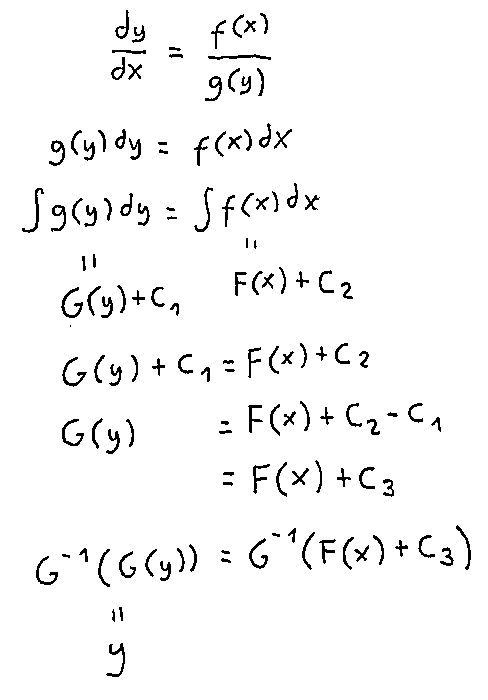
\includegraphics[height=7.5cm]{2020-2-C2/20210416_edovs_caso_geral.pdf}
 }
 \right)
$

\newpage

Digamos que queremos resolver esta EDO:
%
$$\dydx = -\frac{x}{y}$$

Aparentemente dá pra resolvê-la usando
%
$$\pfo{EDOVSG}\bmat{f(x):=-x \\ g(y):=y}\;,$$

mas também precisamos das primitivas $F(x)$ e $G(y)$,

e da inversa $G^{-1}(y)$... a substituição certa é:
%
$$\pfo{EDOVSG}
  \bmat{f(x):=-x \\
        g(y):=y \\
        F(x) := -\frac{x^2}{2} \\
        G(y) := \frac{y^2}{2} \\
        G^{-1}(z) := \sqrt{2z} \\
       }
$$

\newpage

$\text{...que dá isto:}
  \qquad
  % (find-latexscan-links "C2" "20210416_edovs_circulos")
  % (find-xpdf-page "~/LATEX/2020-2-C2/20210416_edovs_circulos.pdf")
  \myvcenter{
  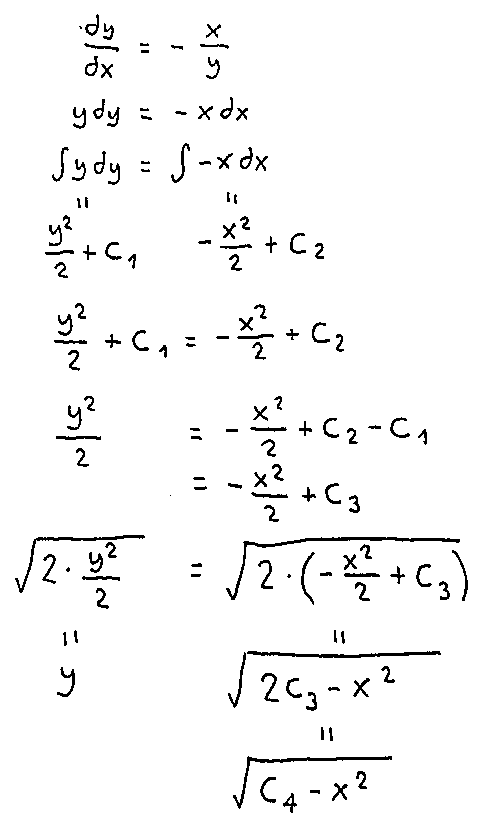
\includegraphics[height=7cm]{2020-2-C2/20210416_edovs_circulos.pdf}
  }
$

(As últimas linhas têm passos extras.)


\newpage

% «como-testar-uma-sol»  (to ".como-testar-uma-sol")
% (c2m202edovsp 11 "como-testar-uma-sol")
% (c2m202edovsa    "como-testar-uma-sol")

{\bf Como testar uma solução}

Digamos que estamos tentando resolver a EDO
%
$$\begin{array}{rcll}
  f'(x) &=& \D -\frac{x}{f(x)}, & \qquad\text{ou:} \\[10pt]
  \D \dydx &=& \D -\frac{x}{y}  \\
  \end{array}
$$

e queremos ver se estas duas funções são solução dela:

$f_1(x) = x^2 + 3$, $f_2(x) = \sqrt{25-x^2}$.

\newpage

{\bf Como testar uma solução (2)}

Basta fazer:
%
$$\scalebox{0.85}{$
  \begin{array}{rcll}
  \left( f'(x) = \D -\frac{x}{f(x)} \right)
  \; \bmat{ f(x) := x^2 + 3 \\ f'(x) = 2x }
  &=&
  \left( 2x = \D -\frac{x}{x^2+3} \right)
  \\[15pt]
  \left( f'(x) = \D -\frac{x}{f(x)} \right)
  \; \bmat{ f(x) := \sqrt{25-x^2} \\ f'(x) = \frac{-x}{\sqrt{25-x^2}} }
  &=&
  \left( \D \frac{-x}{\sqrt{25-x^2}} = \D -\frac{x}{\sqrt{25-x^2}} \right)
  \\
  \end{array}
  $}
$$

e ver se as igualdades da direita são verdadeiras para todo $x$

no domínio de cada função --- aliás, nos pontos em que a função

é derivável...

\msk

A função $f_1(x)=x^2$ está definida em todo $\R$ e é derivável

em $\R$, e a função $f_2(x) = \sqrt{25-x^2}$ está definida no intervalo

fechado $[-5,5]$ e é derivável no intervalo aberto $(-5,5)$.

\msk

Também dá pra testar soluções gerais, basta tratar os `$C$'s

delas como constantes.

\newpage

% «exercicio-3»  (to ".exercicio-3")
% (c2m202edovsp 13 "exercicio-3")
% (c2m202edovsa    "exercicio-3")

{\bf Exercício 3.}

No exercício 1g você desenhou o campo de direções desta EDO:
%
$$ \frac{dy}{dx} = - \frac{y}{x} \qquad (**)$$

e pelo campo de direções você deve ter conseguido ter uma noção

de quais são as soluções dela... (dica: hipérboles!)

\msk

a) Resolva a EDO $(**)$ fazendo isto aqui:
%
$$\pfo{EDOVSG}
  \bmat{f(x) = -1/x \\
        g(y) = 1/y \\
        F(x) = \Rd{?} \\
        G(y) = \Rd{?} \\
        G^{-1}(y) = \Rd{?} \\
        }
$$

(Dica: preencha os `$\Rd{?}$'s corretamente)

\newpage

{\bf Exercício 3.}

b) Diga qual é a solução geral.

c) Teste a sua solução geral.

d) Obtenha a solução que passa pelo ponto $(2,3)$.

e) Obtenha a solução que passa pelo ponto $(2,-2)$.



\newpage


{\bf Funções inversas por chutar e testar}

Digamos que 
%
$$\begin{array}{rcl}
  y &=& 3 + \sqrt{x+4}, \quad \text{isto é}, \\
  f(x) &=& 3 + \sqrt{x+4},
  \end{array}
$$

e sejam:
%
$$\begin{array}{rcl}
  g(y) &=& (y-3)^2 + 4, \\
  h(y) &=& (y-4)^2 + 3. \\
  \end{array}
$$

Eu acho difícil ver só fazendo contas de cabeça se $f^{-1}(y) = g(y)$
ou se $f^{-1}(y) = h(y)$... então é bom a gente saber testar se as
inversas que a gente obteve de cabeça estão certas. O teste é:
%
$$\begin{array}{rcl}
  (f^{-1}(f(x)) = x) \bsm{ f(x) := 3 + \sqrt{x+4} \\ f^{-1}(y) := (y-3)^2 + 4 } &=& \ColorRed{?} \\
  (f^{-1}(f(x)) = x) \bsm{ f(x) := 3 + \sqrt{x+4} \\ f^{-1}(y) := (y-4)^2 + 3 } &=& \ColorRed{?} \\
  \end{array}
$$


\newpage


{\bf Funções inversas por chutar e testar (2)}

O modo tradicional de obter inversas é por

uma série de passos, como:
%
$$\begin{array}{rcl}
  f(x) &=& 3 + \sqrt{x+4} \\
  y &=& 3 + \sqrt{x+4} \\
  y - 3 &=& \sqrt{x+4} \\
  (y - 3)^2 &=& x+4 \\
  (y - 3)^2 - 4 &=& x \\
  (y - 3)^2 - 4 &=& f^{-1}(y) \\
  \end{array}
$$

...mas é importante a gente saber testar se

chegou na inversa certa.


\newpage

% «exercicio-4»  (to ".exercicio-4")
% (c2m202edovsp 17 "exercicio-4")
% (c2m202edovsa    "exercicio-4")

{\bf Exercício 4.} 

Obtenha inversas para as seguintes funções:

%
$$\begin{array}{rcl}
  f_1(x) &=& 2 + 3 \sqrt   {5x+6} \\
  f_2(x) &=& 2 + 3 \sqrt[4]{5x+6} \\
  f_3(x) &=& 2 + 3 (4x+5)^6 \\
  f_4(x) &=& 2 + 3 \ln(4x + 5) \\
  f_5(x) &=& 2 + 3 e^{4x + 5} \\
  f_6(x) &=& \sqrt{2 + 3 e^{4x + 5}} \\[10pt]
  f_7(x) &=& \ln x \\
  f_8(x) &=& \ln -x\\
  f_9(x) &=& |x|\\
  f_{10}(x) &=& \ln |x|\\
  \end{array}
$$

\msk

Porque é que $f_9^{-1}(x)$ e $f_{10}^{-1}(x)$ não existem?


\newpage


{\bf Resolvendo ``direto''}

No segundo vídeo sobre esta parte da matéria -- este aqui:

\ssk

{\footnotesize

\url{http://angg.twu.net/eev-videos/2020-2-C2-edovs-2.mp4}

}

\ssk

eu comecei mostrando como resolver a EDO $$\frac{dy}{dx} = - \frac xy,$$

depois passei pro caso geral, $$\frac{dy}{dx} = \frac{f(x)}{g(y)},$$

e aí defini o ``método'' $\pfo{EDOVSG}$... e nos exercícios

que vieram depois disso nós usamos o $\pfo{EDOVSG}$

e a operação `$[:=]$'.


\newpage

% «exercicio-5»  (to ".exercicio-5")
% (c2m202edovsp 18 "exercicio-5")
% (c2m202edovsa    "exercicio-5")

{\bf Exercício 5.}

a) Tente resolver esta EDO ``direto'',

como no início do vídeo:
%
$$\frac{dy}{dx} = \frac{1}{2y}$$

E pare quando você chegar neste ponto:
%
$$y^2 = x + C_4$$

O passo seguinte, se seguirmos o método do vídeo, é
%
$$y = \ColorRed{±}\sqrt{x + C_4}...$$

\newpage

{\bf Exercício 5 (cont.)}

Podemos considerar que temos duas soluções gerais:
%
$$\begin{array}{rcl}
  f_1(x) &=& \ColorRed{+}\sqrt{x + C_4}, \quad \text{e} \\
  f_2(x) &=& \ColorRed{-}\sqrt{x + C_4}. \\
  \end{array}
$$

b) Encontre o valor que $C_4$ que faz com que $f_1(2)=3$.

c) Encontre o valor que $C_4$ que faz com que $f_2(4)=-5$.

d) Encontre a solução que passa pelo ponto $(-3,-4)$.


%\printbibliography

\GenericWarning{Success:}{Success!!!}  % Used by `M-x cv'

\end{document}

%  ____  _             _         
% |  _ \(_)_   ___   _(_)_______ 
% | | | | \ \ / / | | | |_  / _ \
% | |_| | |\ V /| |_| | |/ /  __/
% |____// | \_/  \__,_|_/___\___|
%     |__/                       
%
% «djvuize»  (to ".djvuize")
% (find-LATEXgrep "grep --color -nH --null -e djvuize 2020-1*.tex")

 (eepitch-shell)
 (eepitch-kill)
 (eepitch-shell)
# (find-fline "~/2020.2-C2/")
# (find-fline "~/LATEX/2020-2-C2/")
# (find-fline "~/bin/djvuize")

cd /tmp/
for i in *.jpg; do echo f $(basename $i .jpg); done

f () { rm -fv $1.png $1.pdf; djvuize $1.pdf }
f () { rm -fv $1.png $1.pdf; djvuize WHITEBOARDOPTS="-m 1.0" $1.pdf; xpdf $1.pdf }
f () { rm -fv $1.png $1.pdf; djvuize WHITEBOARDOPTS="-m 0.5" $1.pdf; xpdf $1.pdf }
f () { rm -fv $1.png $1.pdf; djvuize WHITEBOARDOPTS="-m 0.25" $1.pdf; xpdf $1.pdf }
f () { cp -fv $1.png $1.pdf       ~/2020.2-C2/
       cp -fv        $1.pdf ~/LATEX/2020-2-C2/
       cat <<%%%
% (find-latexscan-links "C2" "$1")
%%%
}

f 20210416_edovs_caso_geral
f 20210416_edovs_circulos




%  __  __       _        
% |  \/  | __ _| | _____ 
% | |\/| |/ _` | |/ / _ \
% | |  | | (_| |   <  __/
% |_|  |_|\__,_|_|\_\___|
%                        
% <make>

 (eepitch-shell)
 (eepitch-kill)
 (eepitch-shell)
# (find-LATEXfile "2019planar-has-1.mk")
make -f 2019.mk STEM=2020-2-C2-edovs veryclean
make -f 2019.mk STEM=2020-2-C2-edovs pdf

% Local Variables:
% coding: utf-8-unix
% ee-tla: "c2m202edovs"
% End:
